\documentclass[12pt]{article}
\usepackage[margin=1in]{geometry}
\usepackage{listings}
\usepackage{color}
\usepackage{tikz-qtree}
\usetikzlibrary{chains}
\usepackage[europeanresistors,americaninductors]{circuitikz}
\usepackage{tikz}
\usetikzlibrary{arrows.meta}
\usetikzlibrary{fit}


\definecolor{dkgreen}{rgb}{0,0.6,0}
\definecolor{gray}{rgb}{0.5,0.5,0.5}
\definecolor{mauve}{rgb}{0.58,0,0.82}


\lstset{frame=tb,
  language=Perl,
  aboveskip=3mm,
  belowskip=3mm,
  showstringspaces=false,
  columns=flexible,
  basicstyle={\small\ttfamily},
  numbers=none,
  numberstyle=\tiny\color{gray},
  keywordstyle=\color{blue},
  commentstyle=\color{dkgreen},
  stringstyle=\color{mauve},
  breaklines=true,
  breakatwhitespace=true,
  tabsize=3
}

%Gummi|065|=)
\title{\textbf{Overview of the Bitcoin Cryptocurrency System}}
\author{Siddharth Agarwal\\
	MA 437 Final Paper}

\date{\today}
\begin{document}

\maketitle

\section{Introduction}

The Bitcoin system, as introduced by Satoshi Nakamoto in his seminal paper, has permanently changed the way that we view currency today. Compared to a fiat currency such as gold, whose value is inherent to the substance used, Bitcoin's value is only dependent on the trust of the people who use it. Working as a decentralized P2P cryptocurrency, it is supported only by the nodes currently on the network. In society and pop culture, it has become a symbol for those who think the government plays too much of a role in their citizens' lives. Bitcoin does not require the identities of its users to be disclosed, nor does the public ledger that records all transactions expose any personal characteristics. The system is completely autonomous, in the sense that no one entity has control over the system. In this paper, we will explore the way that this system is architected.

\section{Currency}
A currency's value is dependent on the users. If all trust in the US dollar were to fail on a certain day, the value would fall relative to other currencies. The Bitcoin conversion rate operates on the same principle. A time series of USD/Bitcoin would show large fluctuations over time, with more volatility than any other major currency pair. However, the continued value of Bitcoin is a testament to its ability to stand out among the plethora of cryptocurrencies that have existed before/after Bitcoin. To purchase Bitcoin all one has to do is create a wallet, use a coin provider (such as Coinbase or Circle), and exchange US Dollars for Bitcoin at the current exchange rate (359.50 USD to 1 Bitcoin at the time of writing). A Bitcoin wallet has a unique address associated with the Bitcoins in one's possession. Transferring the Bitcoins to another individual involves knowing their wallet address. This action can be accomplished through any Bitcoin client. The transaction is then posted on a public ledger, known as the Block chain. Although this sounds simple, a complicated system exists behind the scenes to ensure the integrity of payments. If it were to fail, Bitcoins could be spent more than once, destroying the value.

\section{Overview}
Bitcoin is built upon a proof-of-work system, where participants in the system have to complete a certain time-consuming task and that other participants can verify. In this case, it is applied to the block chain. The block chain is a record of all transactions that have ever occurred on the Bitcoin network. As part of the decentralized theme, no one entity has control over the information in it. Because the block chain is only supported by the nodes currently on the network running bitcoin software, Bitcoin is known as a P2P  decentralized system. In the next section, we will explore the reasoning why Bitcoin is known as a cryptocurrency.


\section{Crypographic Hash Functions}
Hash functions take an arbitrary input and compute an output of a fixed size. These functions have a couple properties that make them useful: retrieving the original message is difficult (pre-image resistance), finding two messages with the same hash is rare (collision resistance), and it is difficult to guess a message by repeatedly hashing different messages (second pre-image resistance). They have many applications spanning many industries, including digital signatures, password checking, and messaging.

Cryptographic hash functions are used for a couple purposes in the Bitcoin architecture. Two of the main ones are to sign off on transactions using digital signatures and to compute wallet addresses. The two functions used are SHA-256 and RIPEMD-160. To create a bitcoin address, an encoding of SHA-256 is applied and then an encoding of RIPEMD-160 is applied to the output of the previous hash.

First, we will explore how SHA-256 works. For a message $ M $, there are series of steps that are taken to encode the message. First, if the number of bits of $M$, denoted $l$, is not a multiple of 512 or 1024, it is padded using the following formula:
Append the bit "1" to the end of the message, followed by $k$ zero bits, where $k$ is the smallest nonnegative solution to the equation $l+1+k=448 \bmod 512 $. Then, a 64-bit block corresponding to the binary representation for $l$ is appended. The result of this is a padded message whose length is a multiple of 512. The padded message is then split into $N$ 512-bit blocks.

The hash computation on the padded message is now performed for each 512-bit block. There are eight 32-bit constants used, corresponding to the first 32 bits of the fractional parts of the square roots of the first eight prime numbers. Eight working variables, $a...h$, are initialized with these hash values. Then a loop is initialized from $t=0..63$ where the values of $a...h$ are switched around using six logical functions, which all take 32-bit words as inputs and output 32-bit words.

After this is completed, $N$ times, we get a 256-bit message $M$ which is composed of 8 32-bit strings. As you can see, this is a computationally intensive process.

\section{Merkle Trees}
Merkle trees are used by the block chain to keep track of transactions. We build a tree from the leaves upwards, ie. pairs of hashes are concatenated, so that if we have $N$ leaves on one level, we will have $N/2$ nodes on the next level. If a level has an odd number of nodes, a transaction is concatenated with itself. This occurs until we get to the top of the tree. The root node will have a hash that verifies all of the transactions below it. If any transaction is changed, the Merkle root hash will not be the same as the original. This is why each block contains the Merkle root hash, so any transaction can be verified quickly, just by concatenating a sibling branch and moving up the tree. The diagram below shows a simple Merkle tree for a group of four transactions. The hash value belonging to the root at the top is dependent on all four transactions. Any small change in the values of the transactions can immediately be identified by comparing hash values to the original.

\begin{center}
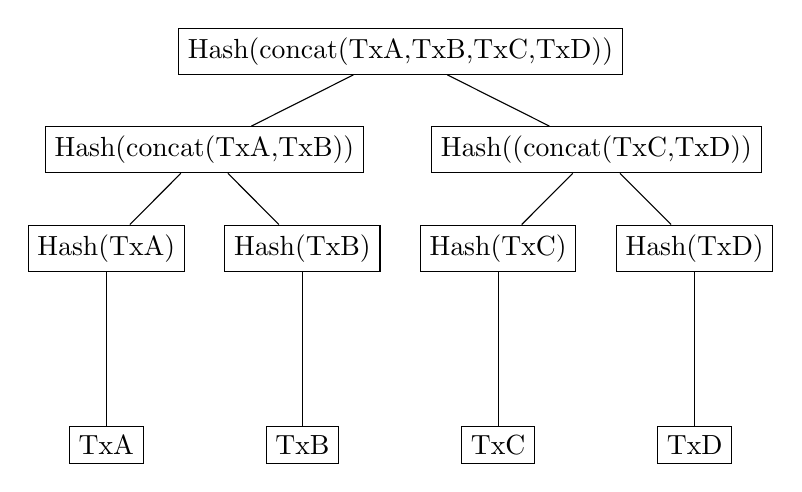
\begin{tikzpicture}[every tree node/.style={draw,rectangle},
   level distance=1.25cm,sibling distance=.5cm,
   edge from parent path={(\tikzparentnode) -- (\tikzchildnode)}]
\Tree [.\node {Hash(concat(TxA,TxB,TxC,TxD))};
    [.Hash(concat(TxA,TxB))
      [.Hash(TxA)
      	[TxA ]
      ]
      [.Hash(TxB)
      	[TxB ]
      ]
    ]
    [.Hash((concat(TxC,TxD))
      [.Hash(TxC)
      	[TxC ]
      ]
      [.Hash(TxD)
      	[TxD ]
      ]
    ]]
\end{tikzpicture}
\end{center}

The hashing algorithm used is SHA-256, performed twice. One theory behind why the double hash was chosen is related to a weakness found in SHA-1. An exploit was found that weakened it to $O(2^{64})$ compared to the designed $O(2^{80})$. One way to harden the algorithm is to double hash, even though such an exploit does not exist for SHA-256. Another theory is that the double hash was chosen is to protect against length extension attacks. This sort of attack has to do with reconstructing the values for the internal variables described in the explanation of SHA-256. Once these are obtained, the message can be extended.


\section{Blockchain Overview}

The way that messages are published to the block chain conforms to a Dynamic Membership Multiparty Signature (DMMS) architecture. We can also describe the design scheme of the block chain as a distributed consensus, which means it adheres to certain properties. Nodes on the network ``lack identities and  join and leave the network at any time, at no cost, without any third parties' permission.''
In the case of Bitcoin, DMMS network participants are known as \textit{miners}.

Each participant on the network keeps a record of the block chain at all times. For a block $B$ that is part of the chain, the header consists of:\begin{itemize}
\setlength\itemsep{.1em}
  \item Version
  \item hash(previous block $A$)
  \item hash(Merkle Root)
  \item Time
  \item Bits: target value for hash($B$)
  \item Nonce: the value that miners are trying to find so that hash($B$) < bits
\end{itemize}

\section{Block chain Mechanics}

Miners work on new groups of transactions called 'blocks', which chain on to the previous blocks in the block chain. A valid block created will receive a lock, and will be chained on to the last block. The longest chain will always be assumed to be the correct one, which forces anyone trying to create a fraudulent block to recreate the entire block chain. The incredibly high CPU time required to do this makes this sort of attack theoretically impossible. Even if one were to start creating a chain, it would be ignored by the other nodes on the network for the purposes of chaining new blocks, since it would be shorter than the real one. The only way that such an attack is possible is if an entity were to gain access to more than 50\% of the network's computing capacity.

The Bitcoin user interface gives the impression that Bitcoins exist in a user's wallet, when really, they exist as the inputs/outputs of transactions. These transactions are at the core of how Bitcoin chains its blocks together, since the hash of the previous block is stored in the next block. The diagram below shows a snapshot of a couple of block headers of a block chain.

\begin{center}
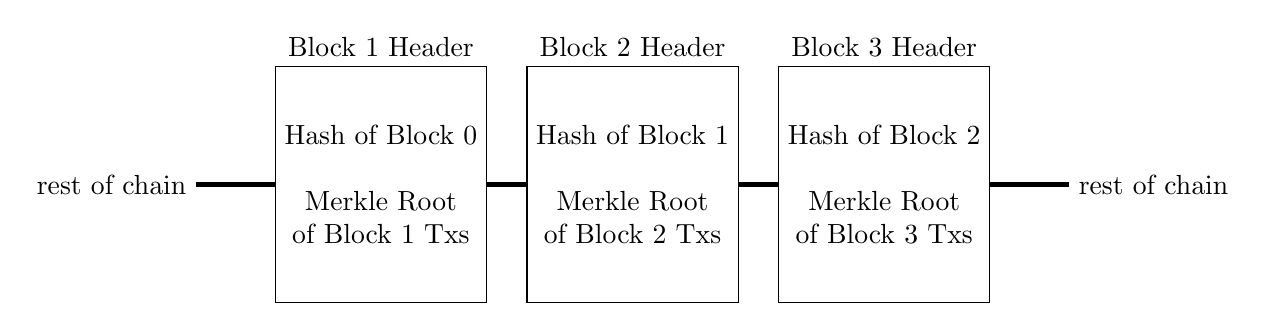
\begin{tikzpicture}[
	start chain=going right,
	box/.style={
		on chain,join,draw,
		minimum height=3cm,
		text centered,
		minimum width=2cm,
	},
	every join/.style={ultra thick},
	node distance=5mm
]
\node [on chain] {rest of chain};
\node [box,xshift=5mm,label=above:Block 1 Header,align=center] (ic) {
    Hash of Block 0\\\\Merkle Root \\of Block 1 Txs
};
\node [box,label=above:Block 2 Header,align=center] {
Hash of Block 1\\\\Merkle Root \\of Block 2 Txs
};
\node [box,label=above:Block 3 Header,align=center] {
Hash of Block 2\\\\Merkle Root\\of Block 3 Txs
};
\node [on chain,join,xshift=5mm]{rest of chain};
\end{tikzpicture}
\end{center}

Miners are incentivized by two things: new Bitcoins created and transaction fees whenever Bitcoins are sent over the network. However, even after the theoretical cap for the number of Bitcoins has been reached (estimated to be around 2140), the other incentive will always remain.

Essentially, the difficulty of creating a block comes from trying to find the 'nonce', or the number that when hashed, will be lower than the difficulty target. The fact that the target is not a set value means that it can be adjusted to correspond to the mining power on the network. When this value is found, the miner can add that block to the block chain and is rewarded. Because of the difficulty of this task, miners will sometimes create groups to which they will donate their CPU time. When a new block is found by anyone in the group, the incentive will be split among everyone.

We now demonstrate the process of finding a nonce that satisfies a certain criteria, in this case three initial 0's, with a Perl 6 script. As you can see, it takes 1322 iterations to find a string with a suitable hash. Of course, in reality this problem would be much more CPU-intensive.

\section{Code Demonstration}
Perl6 code:
\begin{lstlisting}
use Digest::SHA;

sub buf_to_hex { [~] $^buf.list».fmt: "%02x" }
my $initString = "abc";
my $increment = 1;
my $hexString = buf_to_hex sha256 ($initString ~ $increment).encode: 'ascii';

while !($hexString.substr(0,3) ~~ m/ 000 /) {
  ++$increment;
  $hexString = buf_to_hex sha256 ($initString ~ $increment).encode: 'ascii';
}
\end{lstlisting}
\lstset{language=}
Output:
\begin{lstlisting}
Found hexString "000213955c51ad382c14a1634987938c793bb005b6106a3943a16795b65227cd" using original string "abc1322"
\end{lstlisting}

\section{Conclusion}

Bitcoin has come under criticism recently, mainly for the volatility of its value, and the immense use of electricity to create the currency. However, something that no one is debating are the concepts at the center of Bitcoin, specifically the cryptography and other linear algebra concepts that come together to make this a very robust system that has proven itself to be very resistant to attack or failure.

\begin{thebibliography}{9}
\bibitem{devguide}
"Bitcoin Developer Guide"
\textit{Bitcoin.org}.
N.p., n.d. Web. 6 Dec. 2015.
\\\texttt{https://bitcoin.org/en/developer-guide}

\bibitem{hashcash}
"Hashcash"
\textit{Bitcoin Wiki}.
N.p., n.d. Web. 5 Dec. 2015.
\\\texttt{https://en.bitcoin.it/wiki/Hashcash}

\bibitem{distconsensus}
Jämthagen, Christopher. "Distributed Consensus / The Blockchain." (n.d.): n. pag. Lund University, 12 May 2015. Web. 5 Dec. 2015.
\\\texttt{https://www.control.lth.se/media/Staff/JohanEker/introduction\_to\_cloud\_computing/blockchain.pdf}

\bibitem{hashcash2}
Kartaltepe, Erhan. "Properties of Secure Hash Functions." Denim Group. N.p., n.d. Web. 8 Dec. 2015.
\\\texttt{http://www.denimgroup.com/know\_artic\_secure\_hash\_functions.html}

\bibitem{hashcash}
"Merkle Tree."
\textit{Bitcoin Glossary}.
N.p., n.d. Web. 8 Dec. 2015.
\\\texttt{https://bitcoin.org/en/glossary/merkle-tree}

\bibitem{hashcash}
Meyer, Christopher. "Hash Length Extension Attacks."
\textit{Java Code Geeks}.
N.p., 30 July 2012. Web. 7 Dec. 2015.
\\\texttt{http://www.javacodegeeks.com/2012/07/hash-length-extension-attacks.html}

\bibitem{hashcash}
Mironov, Ilya.
\textit{Hash Functions: Theory, Attacks, and Applications}.
Microsoft Research, 14 Nov. 2005. Web. 3 Dec. 2015.
\\\texttt{http://research.microsoft.com/pubs/64588/hash\_survey.pdf}

\bibitem{hashcash}
Nakamoto, Satoshi. "Bitcoin: A Peer-to-Peer Electronic Cash System." Web. 4 Dec. 2015.
\\\texttt{https://bitcoin.org/bitcoin.pdf}

\bibitem{hashcash}
"Proof of Work."
\textit{Bitcoin Wiki}.
N.p., n.d. Web. 10 Dec. 2015.
\\\texttt{https://en.bitcoin.it/wiki/Proof\_of\_work}

\bibitem{hashcash}
"Protocol Documentation."
\textit{Bitcoin Wiki}.
N.p., n.d. Web. 8 Dec. 2015.
\\\texttt{https://en.bitcoin.it/wiki/Protocol\_documentation}

\bibitem{hashcash}
"Secure Hash Standard (SHS)."
\textit{National Institute of Standards and Technology.}
U.S. Department of Commerce, Mar. 2012. Web. 7 Dec. 2015
\\\texttt{http://csrc.nist.gov/publications/fips/fips180-4/fips-180-4.pdf}



\end{thebibliography}

\end{document}
